\section{Approach}
\label{sec:approach}
Opinion summarization is to generate abstractive 
summary expressing salient opinions of multi-review.
As taking textual multi-reviews or structured opinion-aspect pairs as input always causes the generated summary to lose important information,
we construct a semi-structured input and summarize it by summarization models.


\subsection{Semi-structured Data}
\label{sec:data}
Given the textual version of the inputs in synthetic dataset,
we create a semi-structured (input, output) pair
by extracting opinion-aspect pairs (OAs) and 
implicit sentences (ISs) from the textual input as semi-structured input and
taking its corresponding summary as output.

%\textbf{Opinion-aspect Pairs Extraction.} 
We first utilize a rule-based MIN-MINER ~\cite{basicOpiMin20} to get the dependency parse trees of sentences and then use a set of syntactic rules~\cite{aspect12} to extract the OAs.
Meanwhile, we collect the sentences that cannot extract OAs from as the ISs.


\subsection{Summarization Models}
\label{sec:model}
Given semi-structured input,
we add the {\em special token} $[SEP]$ to the beginning of the OAs and concatenate them in a shuffled order. 
For example, the OAs in \tabref{tab:previous_data} with special tokens is represented as:
\begin{example}
	\label{ex:exp}
	%\fbox{
	%\parbox{0.9\columnwidth}{
	\small{``...[SEP] amazing price [SEP] very good food [SEP] generous portions [SEP] poor service... ''} 
	%}}
\end{example}
The ISs are concatenated in the same way as OAs. 
We express the sequence of tokens in OAs as  $\textbf{x}^o$=$\{x^o_{0,0},x^o_{1,0},...,x^o_{0,1},...,x^o_{m,M}\}$
and the tokens in ISs as $\textbf{x}^s$=$\{x^s_{0,0},x^s_{1,0},...,x^s_{0,1},...,x^s_{n,N}\}$.
$x^o_{i,j}$ is the $i$-th token of $j$-th OAs.
$x^s_{i,j}$ is the $i$-th token of $j$-th ISs.
$x^o_{0,j}$ and $x^s_{0,j}$ are $[SEP]$.
$y_k$ is the $k$-th token of summary $\textbf{y}$=$\{y_0, y_1,..., y_t\}$.           


\begin{figure}[th]
	\centering
	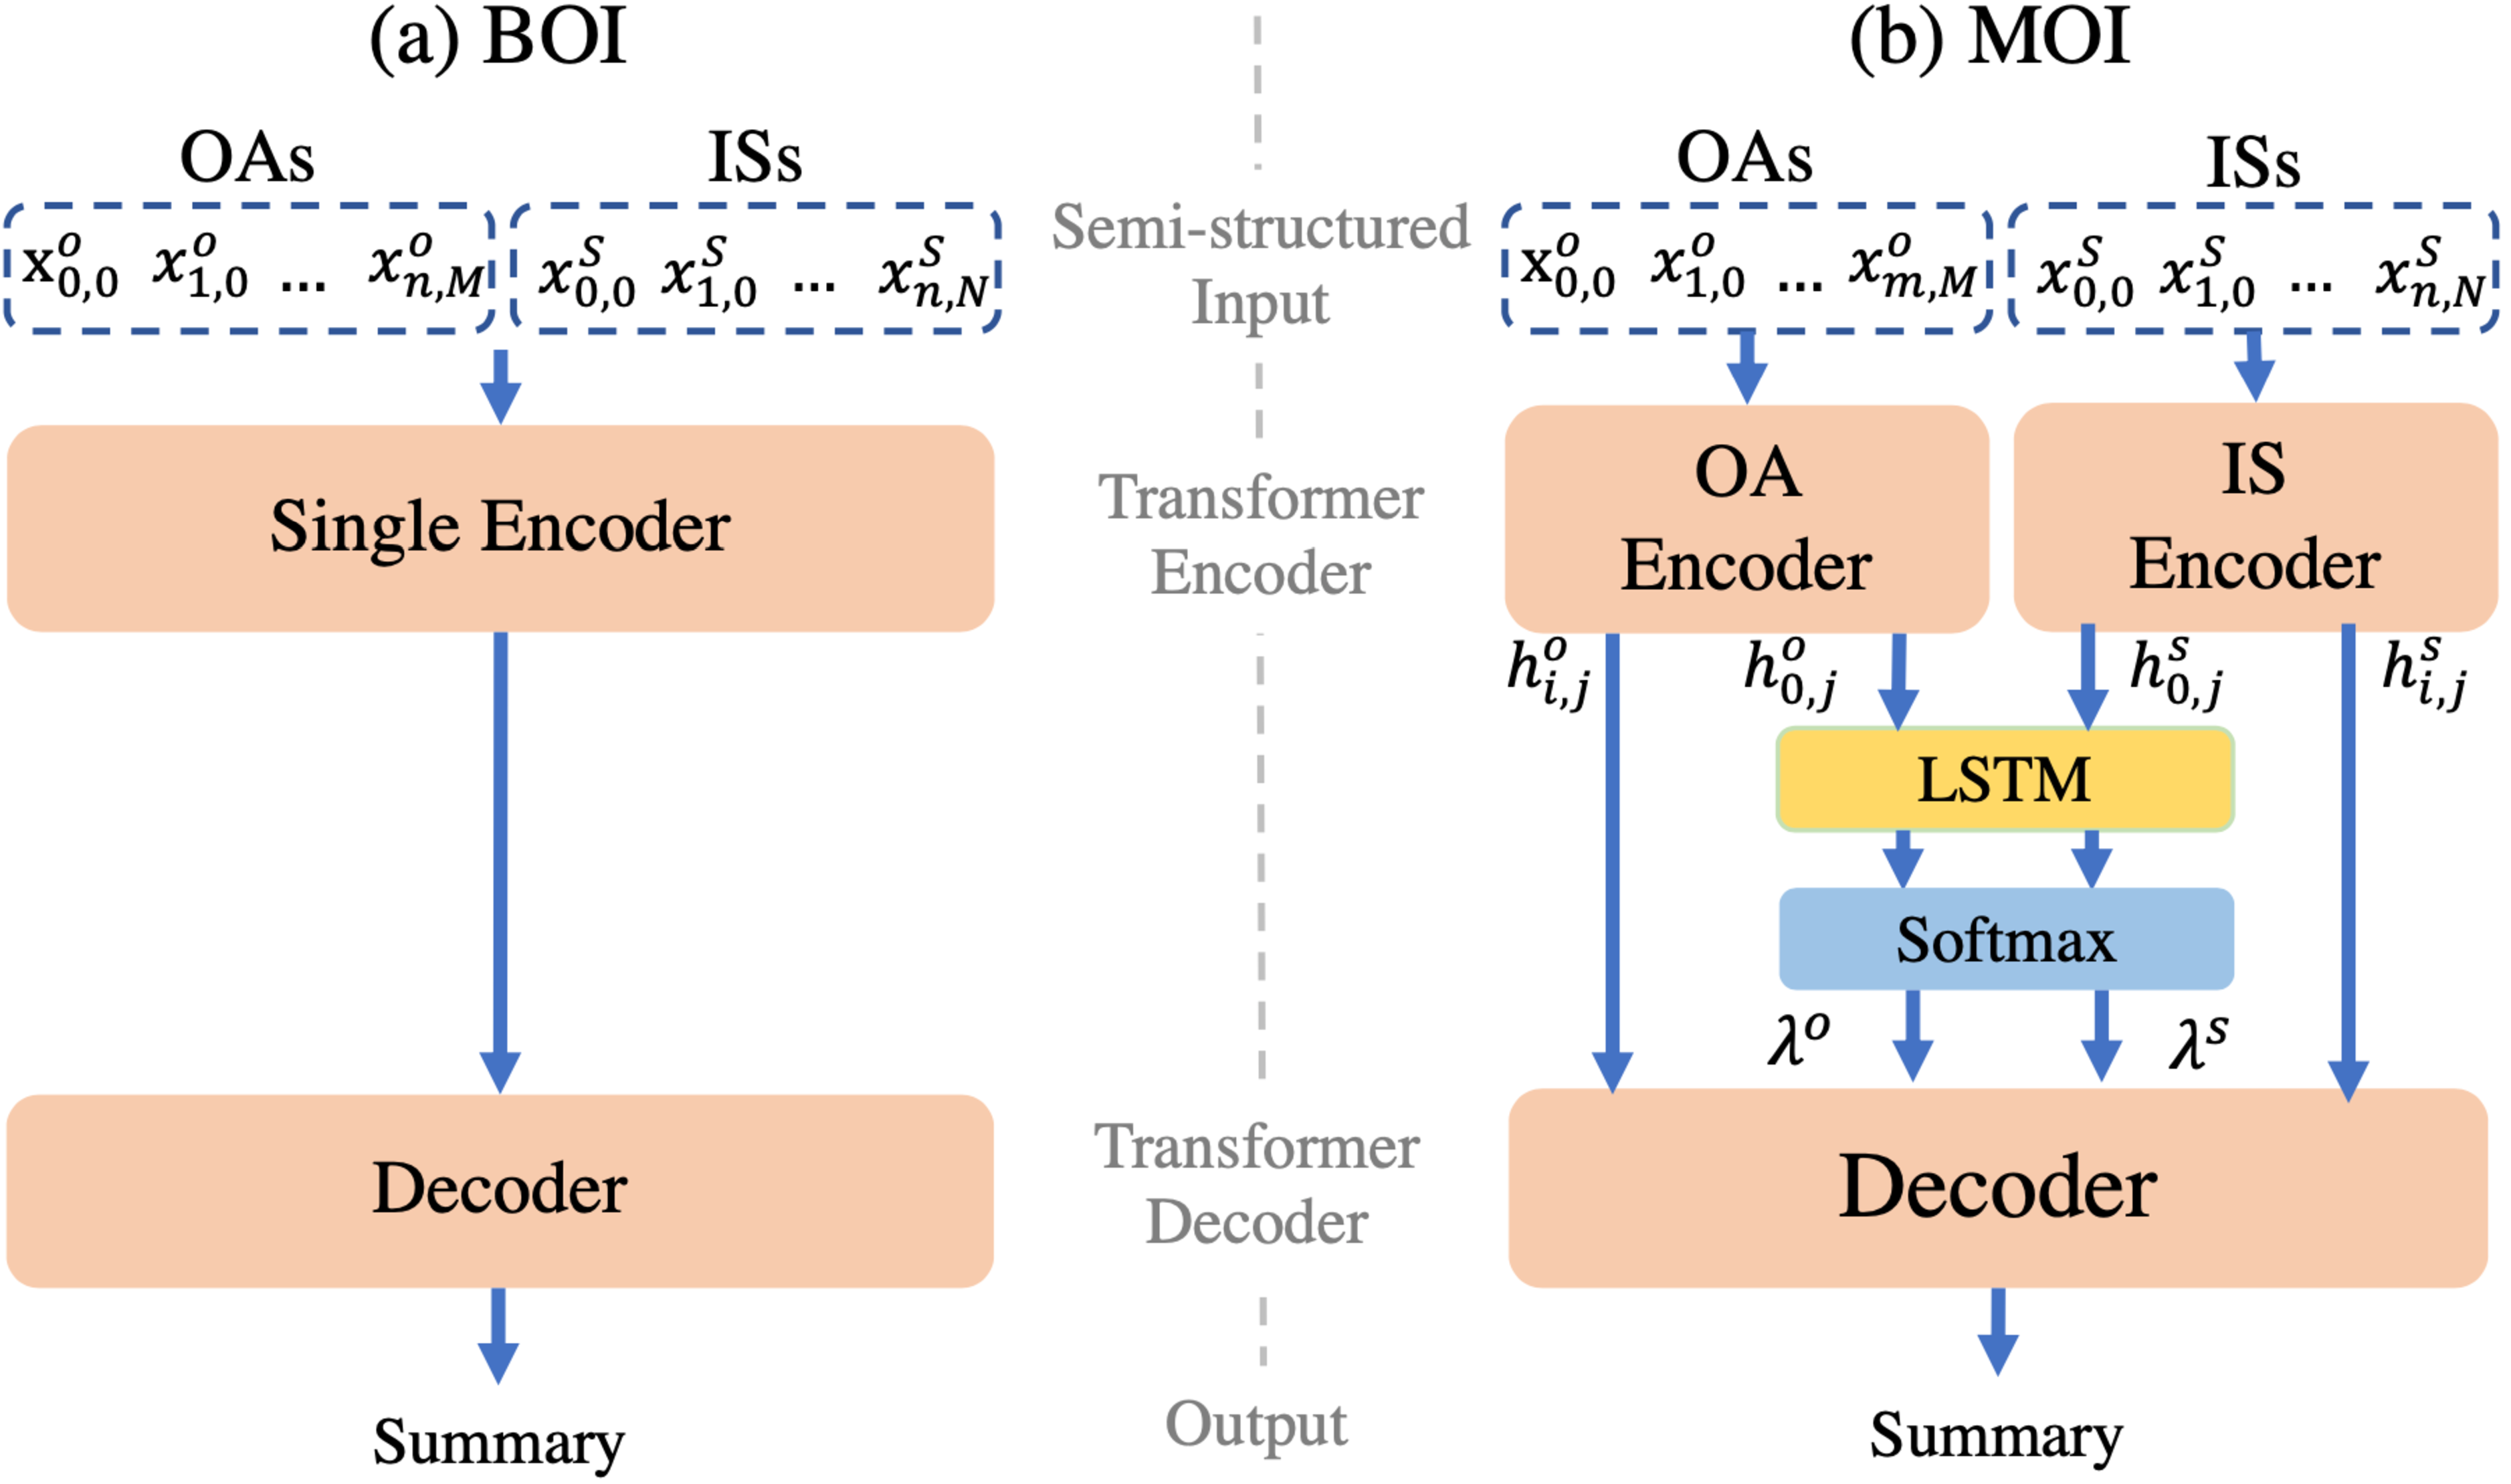
\includegraphics[width=1\linewidth]{./model.pdf}
	\caption{The architecture of our proposed models.}
	\label{fig:model}
\end{figure}       


\subsubsection{Basic Seq2seq Model with OAs and ISs (BOI)} 
BOI concatenates $\textbf{x}^o$ and $\textbf{x}^s$
as input $\textbf{x}^a$=$\{x^o_{0,0},x^o_{1,0},...,x^o_{m,M},x^s_{0,0}, x^s_{1,0},...,\\x^s_{n,N}\}$
for transformer seq2seq model, as shown in \figref{fig:model}(a). 
The goal of BOI is to estimate the conditional probability
$p(\textbf{y}|\textbf{x}^a)$:
\begin{equation}
	%\small
	p(\textbf{y}|\textbf{x}^a) \!=\! 
	{\prod^T_{t} {p(y_{t} | y_{0}, y_{1},..., y_{t-1}, \textbf{x}^a)}}        
\end{equation}
 
We expect OA to enhance
the hightlight of opinion information and IS to complement OA in capturing important information.
Since the structure of OA and IS is different,
we design a modified seq2seq model to handle OAs and ISs through two pipelines respectively.



\subsubsection{Modified Seq2seq Model with OAs and ISs (MOI)}
MOI is a dual-encoder model and handles OAs and ISs
via two transformer encoders, \textbf{\em OA encoder} and \textbf{\em IS encoder}. 
%Both of them are transformer-based encoder.
The architecture is illustrated in \figref{fig:model}(b).

%We use the same methods to get
%noisy OAs embedding $\textbf{x}^p$=$(x^p_{0,0},x^p_{1,0},...,x^p_{u,U})$ 
%and noisy OSs embedding $\textbf{x}^s$=$(x^s_{0,0},x^s_{1,0},...,x^s_{v,V})$.
%We input noisy OAs to OA encoder and noisy ISs to IS encoder.
%$H^p_j$ and $H^s_{j'}$ is the encoder hidden state for $j$-th OA pair
%and $j'$-th IS sentence through LSTM layers.
%We take the last hidden state $H^p_U$ and $H^s_V$
%to represent opinion-aspect (generalized) information 
%and implicit sentences (specific) information.
%We use $h^p_{i,j}$ and $h^s_{i',j'}$ to denote the encoder hidden state for $i$-th words in $j$-th OA pair
%and $i'$-th word in $j'$-th IS sentence.
At each decoding step $t$, 
$\textbf{c}_t^o$ is the context vector of OA encoder, which is the weighted sum of the hidden states of OA 
encoder with Encoder-Decoder Attention (Enc-Dec Attn) as weight. 
$\textbf{c}_t^s$ is the weighted sum of IS encoder hidden states.

Inspired by~\citet{DialogMV2020},
we use the representation of the $j$-th special token, $h^o_{0,j}$,
to describe the information of the $j$-th OA pair in OAs.
We use $h^s_{0,j}$ to represent the $j$-th sentence in ISs.
Then we utilize LSTM ~\cite{LSTM1997}  to respectively 
aggregate the information of all OA pairs
$\{h^o_{0,j}|0\leq{j}\leq{M}\}$ in OAs
and all sentences $\{h^s_{0,j}|0\leq{j}\leq{N}\}$ in ISs by:
\begin{equation}
	%\small
	H^o_j = LSTM(h^o_{0,j}, H^o_{j-1})
\end{equation}
\begin{equation}
	%\small
	H^s_j = LSTM(h^s_{0,j}, H^s_{j-1})
\end{equation}
%The last hidden state $H^p_U$.
%where $H^p_j$ is the encoder hidden state for $j$-th OA.
We use the last state $H^o_M$ and $H^s_N$
to represent the input OAs and ISs.
$\lambda^o$ and $\lambda^s$ denote
the weight of the OAs and ISs,
which are calculated by:
\begin{equation}
	%\small
	\tilde{H}^o_M = \tanh(W^oH^o_M+b^o) 
\end{equation}
\begin{equation}
		%\small
	\tilde{H}^s_N = \tanh(W^sH^s_N+b^s) 
\end{equation}
\begin{equation}
	%\small
    \lambda^o = \frac{\exp(\tilde{H}^o_M {^\top} \textbf{c}_0^o)}{\exp(\tilde{H}^o_M {^\top} \textbf{c}_0^o)+\exp(\tilde{H}^s_N {^\top} \textbf{c}_0^s)} 
\end{equation}
\begin{equation}
%\small
	\lambda^s = 1-\lambda^o 
\end{equation}
where 
%$v^p$ and $v^s$ respectively denote the randomly initialized context vector of OA encoder and IS encoder.
$W$ and $b$ are trainable parameters.
The weighted context vector $\textbf{c}_t$ of 
the semi-structured input is:
\begin{equation}
	%\small
	\textbf{c}_t = \lambda^o \textbf{c}_t^o +  \lambda^s \textbf{c}_t^s
\end{equation}

Thus, the probability of the $t$-th output of the decoder
is:
\begin{equation}
%\small
p(y_t|y_{0}, y_{1},..., y_{t-1},\textbf{x}^o,\textbf{x}^s)=
softmax(W \textbf{c}_t)
\end{equation}





